\section{Introduction}
\label{introduction}
Wind energy is one of the cornerstones of the ongoing transition toward sustainable electricity generation. As wind turbines are deployed in increasingly large farms, both onshore and offshore, the aerodynamic interaction among turbines becomes a critical design and operational challenge. When a turbine extracts kinetic energy from the incoming flow, it leaves behind a wake region characterised by a significant velocity deficit and elevated turbulence levels. Downstream turbines that operate within this region consequently suffer both reduced power output and increased fatigue loads, affecting the economic and structural performance of the entire farm~\cite{Porte-Agel2020}. Accurate prediction of wind turbine wake behaviour is therefore essential for wind farm layout optimisation, energy yield estimation, and structural load assessment.

From a fluid-mechanics perspective, the wake of a horizontal-axis wind turbine (HAWT) is a complex, multi-scale phenomenon. It is deeply coupled with the Atmospheric Boundary Layer (ABL), which is itself inherently unsteady and stratified~\cite{Porte-Agel2020}. The near-wake region, dominated by the tip vortex system shed by the rotor blades, transitions into a far-wake where shear-driven turbulent mixing progressively restores the velocity deficit. This recovery process is strongly influenced by the ambient turbulence intensity, wind shear, thermal stability, and the topography of the terrain~\cite{heck2025unravelingeffectsatmosphericdynamics}. The wide range of length and time scales involved, from blade boundary layers to the full extent of the ABL, makes any single simulation approach inherently challenging.

The reliability of any farm-level study ultimately rests on how faithfully the turbine wakes are reproduced: it is the wake of each machine that sets the inflow, the power output and the fatigue loading of the ones downstream. This requirement, rather than the resolution of the single rotor, is what dictates the computational cost of the simulation. Several modelling strategies are available, each representing a different trade-off between physical fidelity and computational cost. At the low-fidelity end, analytical engineering wake models (e.g., the Jensen top-hat model and its Gaussian successors) offer near-instantaneous evaluation and are therefore routinely used in wind farm layout optimisation~\cite{GholamiAnjiraki2025}, but they rely on strong simplifying assumptions and cannot capture the complex turbulent structure of real wakes. At the high-fidelity end, scale-resolving Computational Fluid Dynamics (CFD) is required whenever the wake physics itself must be predicted.

Figure~\ref{fig:cost_landscape} summarises a bibliographically-grounded, order-of-magnitude \emph{estimate} of the computational cost of such CFD studies for a representative set of single-turbine and wind-farm configurations, in the plane spanned by the total grid size and the number of time steps needed to converge the wake statistics; the diagonals are iso--core-hour lines and the shaded bands mark the corresponding feasibility regimes on a Tier-0 system (CINECA Leonardo). The estimate is not a benchmark measurement: it is built bottom-up from per-turbine cell counts and wake-resolving flow-through times, with a per-cell solver cost calibrated against published blade-resolved runs and converted to energy and economic cost under explicit assumptions. Specifically, the per-turbine meshes follow published practice for the NREL~5~MW -- of order $5\times10^{7}$ cells for blade-resolved URANS~\cite{Sebastiani2024}, up to $\mathcal{O}(10^{9})$ points for blade-resolved LES~\cite{Sharma2024Exawind}, and one to two orders of magnitude fewer for actuator models~\cite{coarseALM2016,Troldborg} -- while the hardware, energy and cost figures assume the CINECA~Leonardo system (the GPU Booster partition for LES and the CPU DCGP partition for URANS)~\cite{Turisini2023Leonardo}, a power-usage effectiveness of $1.2$ and an electricity price of $0.15$~EUR/kWh. Two conclusions follow. First, fully blade-resolved (full-geometry) simulations, which resolve the rotor boundary layers, are confined to the single-turbine regime: extended to a $20$--$40$ turbine farm they exceed the exascale envelope (in excess of $10^{10}$ cells and tens of millions of euros per single run) and are therefore not a viable option for farm-level studies. Wake studies at farm scale are thus affordable only through actuator models (actuator-line or actuator-disk), which replace the blades with body forces and lower the cell count by one to two orders of magnitude while still generating a physical wake. Second, once the actuator simplification is accepted, the residual choice is one of turbulence-modelling fidelity. For reference, the approximate positions of representative high-fidelity studies from the literature are overlaid on the same plane (grey diamonds, labelled by their bibliography number in this paper), spanning from coarse actuator-line LES of single rotors~\cite{coarseALM2016,Troldborg} through actuator wind-farm LES~\cite{Steiner2021,Deskos2018,Joulin2019,Sebastiani2021Lillgrund,Stevens2014,King_2018,alessio5-mw,Carloni2026} to fully blade-resolved single-turbine and array simulations~\cite{Sebastiani2024,Sharma2024Exawind,Kirby2019}.

\begin{figure*}[h]
    \centering
    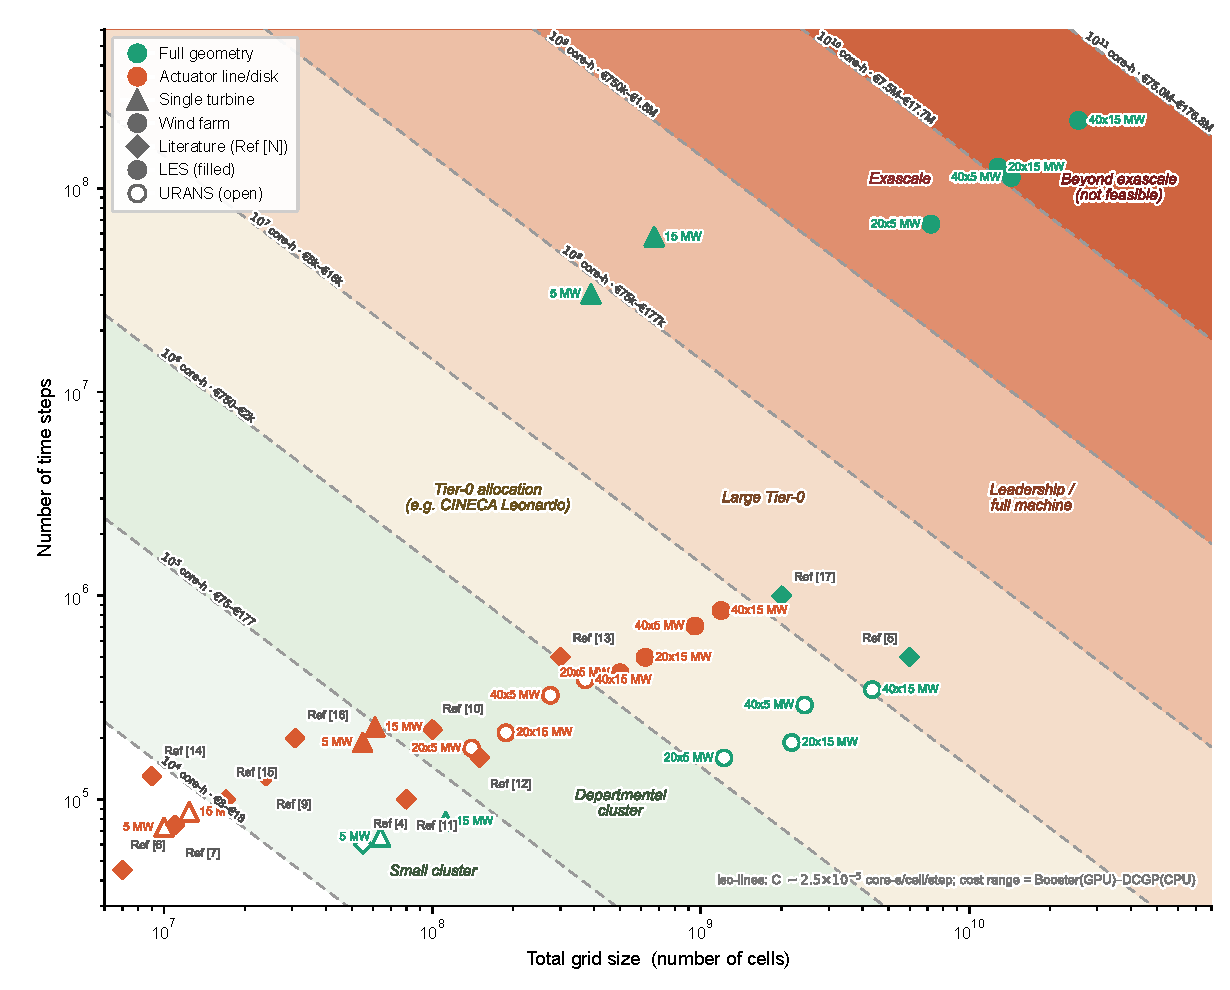
\includegraphics[width=\textwidth]{introduction/img/fig_selection_chart_lit.pdf}
    \caption{Order-of-magnitude computational cost of single-turbine and wind-farm CFD, in the grid-size/time-step plane. Coloured markers distinguish full-geometry (green) from actuator (red) models, single turbines (triangles) from farms (circles), and LES (filled) from URANS (open). Grey diamonds are representative literature studies, annotated with their reference number in this paper's bibliography (approximate placement, order-of-magnitude). Dashed diagonals are iso--core-hour lines (with the associated electricity-cost range on CINECA Leonardo); shaded bands mark the feasibility regimes. Cost-model values are bibliographically-grounded, order-of-magnitude estimates -- not benchmark measurements -- obtained from a bottom-up model calibrated on the mesh and hardware benchmarks cited in the text.}
    \label{fig:cost_landscape}
\end{figure*}

Within the actuator family, unsteady Reynolds-Averaged Navier-Stokes (URANS) is by far the cheapest option and reproduces the integral rotor quantities -- torque, thrust and hence power -- with good accuracy. However, the eddy-viscosity closure on which it relies, with its Boussinesq hypothesis and isotropic treatment of the Reynolds stress tensor, introduces structural model-form errors that are particularly pronounced in separated and wake flows: the turbulent mixing that drives wake recovery is systematically mis-predicted, so that the resulting wake is largely non-physical~\cite{72116acdc5aa4b3b8fc752f1b2fa9958,Moss2023}. Large Eddy Simulation (LES) coupled to the same actuator model resolves the dominant wake structures explicitly and is the reference standard for wake physics, but a single farm-scale simulation can still demand between $10^5$ and $3\times10^6$ CPU hours~\cite{Steiner2021} -- one to two orders of magnitude more than the corresponding URANS. The gap between these two actuator configurations -- the same grid topology, a very different wake fidelity -- is precisely the margin this work targets: the objective is to obtain, on a URANS-actuator grid and at a URANS-actuator cost, a wake prediction whose accuracy approaches that of an LES-actuator simulation.

The cost estimates of Fig.~\ref{fig:cost_landscape} are reported in full in Tab.~\ref{tab:cost_model} and are built as follows. The cell count of each scenario is assembled bottom-up as the number of turbines times a per-turbine mesh plus a shared background ABL mesh, with per-turbine values taken from published practice (of order $6\times10^{7}$ and $3.5\times10^{8}$ cells for blade-resolved URANS and LES of the NREL~5~MW, and $6\times10^{6}$ and $1.5\times10^{7}$ for the corresponding actuator models, scaled by $1.8$ and $1.4$ for the IEA~15~MW). The number of time steps follows from the physical time needed to develop and statistically average the wake -- several domain flow-through times ($6/8/10$ for URANS and $10/12/14$ for LES, at single/$20$-/$40$-turbine scale) -- divided by the time step, itself set by $2^{\circ}$ of rotor azimuth for blade-resolved URANS, by the near-wall CFL limit ($\approx10^{-4}$~s) for blade-resolved LES, and by one finest cell per blade-tip advancement for actuator models. The HPC workload is then $\mathrm{core\text{-}hours}=\mathrm{cells}\times N_\mathrm{steps}\times C/3600$, with a per-cell solver cost $C\approx2\times10^{-4}$ (URANS) and $3\times10^{-5}$~core-s/cell/step (LES), calibrated against a published blade-resolved run ($\sim$16{,}300~CPU-h for $55$~M cells over $\sim$5{,}400 steps). Energy and economic cost finally follow as $\mathrm{node\text{-}hours}\times\mathrm{node\ power}\times\mathrm{PUE}$ and $\times\,0.15$~EUR/kWh, with LES costed on the GPU Booster partition and URANS on the CPU DCGP partition of Leonardo (PUE~$=1.2$, $1$~Booster node~$\approx600$~CPU cores). Applying the same chain to the reported mesh size and time-stepping of representative literature studies yields the reference cases listed at the bottom of Tab.~\ref{tab:cost_model} and overlaid on Fig.~\ref{fig:cost_landscape}.

\begingroup
\scriptsize
\setlength{\tabcolsep}{3pt}
\begin{longtable}{@{}llccrrrr@{}}
\caption{Cost-model scenarios behind Fig.~\ref{fig:cost_landscape} (order-of-magnitude estimates) and the literature reference cases overlaid on it. The calculation chain is detailed in the text.}\label{tab:cost_model}\\
\hline
Case & Configuration & Model & MW & Cells [$10^{6}$] & $N_\mathrm{steps}$ & Core-h & Cost [EUR] \\
\hline
\endfirsthead
\multicolumn{8}{@{}l}{\footnotesize\itshape Table~\ref{tab:cost_model} -- continued} \\
\hline
Case & Configuration & Model & MW & Cells [$10^{6}$] & $N_\mathrm{steps}$ & Core-h & Cost [EUR] \\
\hline
\endhead
\hline
\endfoot
\multicolumn{8}{@{}p{0.96\linewidth}}{\footnotesize $^{\dagger}$~Reference-case core-hours are indicative, computed with the same per-cell solver cost as the cost-model scenarios ($C=2\times10^{-4}$~core-s/cell/step for URANS, $3\times10^{-5}$ for LES); the cells and $N_\mathrm{steps}$ of the reference cases are order-of-magnitude placements (see Fig.~\ref{fig:cost_landscape}).} \\
\hline
\endlastfoot
1 & Single, full-geom. & LES & 5 & 390.0 & $3.0\!\times\!10^{7}$ & 98.3M & 73,710 \\
1 & Single, full-geom. & LES & 15 & 670.0 & $5.8\!\times\!10^{7}$ & 321.6M & 241,200 \\
1 & Single, full-geom. & URANS & 5 & 64.0 & $6.5\!\times\!10^{4}$ & 232k & 411 \\
1 & Single, full-geom. & URANS & 15 & 112.0 & $7.8\!\times\!10^{4}$ & 484k & 855 \\
2 & Single, actuator & LES & 5 & 55.0 & $1.9\!\times\!10^{5}$ & 87k & 65 \\
2 & Single, actuator & LES & 15 & 61.0 & $2.3\!\times\!10^{5}$ & 115k & 86 \\
2 & Single, actuator & URANS & 5 & 10.0 & $7.3\!\times\!10^{4}$ & 41k & 72 \\
2 & Single, actuator & URANS & 15 & 12.4 & $8.7\!\times\!10^{4}$ & 60k & 106 \\
3 & WF-20, full-geom. & LES & 5 & 7,200 & $6.7\!\times\!10^{7}$ & 3,991.7M & 2,993,760 \\
3 & WF-20, full-geom. & LES & 15 & 12,800 & $1.3\!\times\!10^{8}$ & 13,516.8M & 10,137,600 \\
3 & WF-20, full-geom. & URANS & 5 & 1,220 & $1.6\!\times\!10^{5}$ & 10.8M & 19,132 \\
3 & WF-20, full-geom. & URANS & 15 & 2,180 & $1.9\!\times\!10^{5}$ & 23.0M & 40,697 \\
4 & WF-40, full-geom. & LES & 5 & 14,350 & $1.1\!\times\!10^{8}$ & 13,500.5M & 10,125,360 \\
4 & WF-40, full-geom. & LES & 15 & 25,550 & $2.2\!\times\!10^{8}$ & 45,785.6M & 34,339,200 \\
4 & WF-40, full-geom. & URANS & 5 & 2,435 & $2.9\!\times\!10^{5}$ & 39.3M & 69,427 \\
4 & WF-40, full-geom. & URANS & 15 & 4,355 & $3.5\!\times\!10^{5}$ & 83.6M & 147,821 \\
5 & WF-20, actuator & LES & 5 & 500.0 & $4.2\!\times\!10^{5}$ & 1.7M & 1,306 \\
5 & WF-20, actuator & LES & 15 & 620.0 & $5.0\!\times\!10^{5}$ & 2.6M & 1,928 \\
5 & WF-20, actuator & URANS & 5 & 140.0 & $1.8\!\times\!10^{5}$ & 1.4M & 2,452 \\
5 & WF-20, actuator & URANS & 15 & 188.0 & $2.1\!\times\!10^{5}$ & 2.2M & 3,920 \\
6 & WF-40, actuator & LES & 5 & 950.0 & $7.1\!\times\!10^{5}$ & 5.6M & 4,212 \\
6 & WF-40, actuator & LES & 15 & 1,190 & $8.4\!\times\!10^{5}$ & 8.4M & 6,281 \\
6 & WF-40, actuator & URANS & 5 & 275.0 & $3.2\!\times\!10^{5}$ & 5.0M & 8,758 \\
6 & WF-40, actuator & URANS & 15 & 371.0 & $3.9\!\times\!10^{5}$ & 8.0M & 14,066 \\
\hline
\multicolumn{8}{@{}l}{\itshape Literature reference cases (Fig.~\ref{fig:cost_landscape})} \\
\hline
Ref [4] & Single, full-geom. & URANS & -- & 55.0 & $6.0\!\times\!10^{4}$ & 183k$^{\dagger}$ & -- \\
Ref [5] & Single, full-geom. & LES & -- & 6,000 & $5.0\!\times\!10^{5}$ & 25.0M$^{\dagger}$ & -- \\
Ref [6] & Single, actuator & LES & -- & 7.0 & $4.5\!\times\!10^{4}$ & 3k$^{\dagger}$ & -- \\
Ref [7] & Single, actuator & LES & -- & 11.0 & $7.5\!\times\!10^{4}$ & 7k$^{\dagger}$ & -- \\
Ref [9] & Farm, actuator & LES & -- & 24.0 & $1.3\!\times\!10^{5}$ & 26k$^{\dagger}$ & -- \\
Ref [10] & Farm, actuator & LES & -- & 100.0 & $2.2\!\times\!10^{5}$ & 183k$^{\dagger}$ & -- \\
Ref [11] & Farm, actuator & LES & -- & 80.0 & $1.0\!\times\!10^{5}$ & 67k$^{\dagger}$ & -- \\
Ref [12] & Farm, actuator & LES & -- & 150.0 & $1.6\!\times\!10^{5}$ & 200k$^{\dagger}$ & -- \\
Ref [13] & Farm, actuator & LES & -- & 300.0 & $5.0\!\times\!10^{5}$ & 1.2M$^{\dagger}$ & -- \\
Ref [14] & Single, actuator & LES & -- & 9.0 & $1.3\!\times\!10^{5}$ & 10k$^{\dagger}$ & -- \\
Ref [15] & Single, actuator & LES & -- & 17.0 & $1.0\!\times\!10^{5}$ & 14k$^{\dagger}$ & -- \\
Ref [16] & Single, actuator & LES & -- & 30.8 & $2.0\!\times\!10^{5}$ & 51k$^{\dagger}$ & -- \\
Ref [17] & Farm, full-geom. & LES & -- & 2,000 & $1.0\!\times\!10^{6}$ & 16.7M$^{\dagger}$ & -- \\
\end{longtable}
\endgroup


Machine Learning (ML) has emerged as a powerful paradigm to complement or enhance physics-based simulations across several domains of wind energy research. A large body of literature has applied ML to operational tasks such as wind power forecasting from SCADA data~\cite{Infield2022,Moss2023}, predictive maintenance and condition monitoring of turbine components~\cite{Infield2022}, and wind farm layout optimisation using data-driven surrogate models of wake interactions~\cite{GholamiAnjiraki2025,YANG2023119240}. In these applications ML is generally used downstream of a physical model: a CFD or analytical solver first generates the flow field, and ML then post-processes or surrogate-replaces its output to predict power, loads, or optimal configurations.

A conceptually distinct and more recent line of research aims instead to use ML to correct or replace the turbulence closure itself, modifying the governing equations during the simulation. An example of that can be seen in ~\cite{Duraisamy2019} with the proposed FIML (field inversion and machine learning) proposed by Parish \& Duraisamy and the invariant neural-network closure of Ling et al.~\cite{Ling2016}. In the wind energy context, Steiner et al.~\cite{Steiner2021} demonstrated that optimal corrective fields for the turbulence anisotropy tensor and turbulent kinetic energy production can be derived from time-averaged LES data and used to construct a custom RANS closure via sparse symbolic regression, yielding substantially improved wake predictions for multi-turbine configurations at wind-tunnel scale. Similarly, data-driven Gaussian-process corrections to the eddy-viscosity field, trained on single-turbine LES, have shown improved accuracy when deployed in a wind-plant RANS simulation~\cite{King_2018}. More broadly, Steiner~\cite{72116acdc5aa4b3b8fc752f1b2fa9958} showed that combined baseline-RANS plus data-driven correction strategies can outperform standard models for both velocity and turbulent kinetic energy, while acknowledging that larger datasets and more stable numerical implementations are needed before such methods can be applied at industrial scale.

The present work contributes to this emerging research direction, with specific novelty in three respects. First, rather than identifying a global correction to the turbulence model, a clustering algorithm (CA) based on the K-means method is employed to segment the flow domain into physically distinct regions characterised by different wake dynamics, following the decomposition approach introduced in~\cite{Clustering_tieghi,Carloni2026}. This region-aware strategy naturally improves the generalisability and interpretability of the trained models and makes the correction less sensitive to mesh refinement. Second, a Multi-Layer Perceptron (MLP) is trained to predict the local correction $\Delta\nu_t = \nu_{t,eq} - \nu_{t,\mathrm{RANS}}$ between the LES-equivalent eddy viscosity and the RANS baseline, and the resulting data-driven closure is directly embedded into the OpenFOAM PIMPLE solver via a modified turbulence correction loop, enabling its use in fully predictive RANS simulations. Third, the methodology is tested across multiple mesh refinement levels, demonstrating that LES-quality accuracy in wake recovery can be achieved at a computational cost lower than that of standard LES, which is a prerequisite for practical wind farm applications.

It is worth emphasising what distinguishes this approach from the bulk of ML applications in wind energy. Most existing methods employ ML as a post-processing or surrogate tool applied to the output of a turbulence model; the turbulence model itself is left unchanged. Here, the ML component is used to define the turbulence model, to construct, from scratch, a problem-specific eddy-viscosity closure calibrated to reproduce high-fidelity LES statistics. This opens a path towards compact, computationally efficient flow models that could in the future support real-time wind farm monitoring and control, by providing accurate yet computational effective representations of the wake field and its evolution under varying inflow conditions.

The paper is structured as follows. Sec.~\ref{sec:methodology} describes the CFD campaign used to generate the training and testing data, the clustering pipeline, and the MLP architecture and training strategy. Sec.~\ref{sec:case_study} introduces the NREL-5MW reference turbine case study and the computational domain. Results are presented in Sec.~\ref{sec:results}, covering the clustering, the neural network training metrics, and the performance of the ML-based RANS model on coarser grids. Conclusions are drawn in Sec.~\ref{sec:conclusions}.
